\documentclass[]{standalone}

\usepackage{amsmath}
\usepackage{amsfonts}
\usepackage{amssymb}
\usepackage{graphicx}
\usepackage{tikz}
\usepackage{import}
\usepackage[subpreambles=true]{standalone}

\usepackage{tikz}
\usepackage{tikz-3dplot}
\usepackage{tikz_utils}

\usetikzlibrary{calc}
\usetikzlibrary{positioning}
\usetikzlibrary{patterns}
\usetikzlibrary{decorations,backgrounds}

\begin{document}
    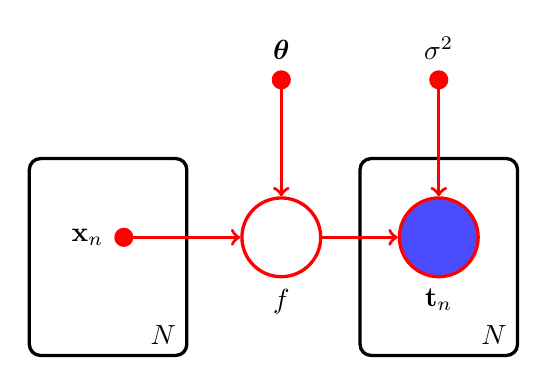
\begin{tikzpicture}[scale=1, very thick]
        % \draw[very thick, red] (0,-2) -- 
        % \draw[very thick, red] (0,0) node[black, left, below]{$f$} circle (0.5cm);
        \draw[rounded corners] (-3.2, 1) rectangle (-1.2, -1.5) node [above left] {$N$};
        \draw[rounded corners] (1, 1) rectangle (3, -1.5) node [above left] {$N$};;
        \node (theta) at (0,2) [shape=circle,draw=red,fill=red, inner sep=0pt, minimum size=2mm,label=north:$\boldsymbol{\theta}$] {};
        \node (sigma) at (2,2) [shape=circle,draw=red,fill=red, inner sep=0pt, minimum size=2mm,label=north:$\sigma^2$] {};
        \node (x) at (-2,0) [shape=circle,draw=red,fill=red, inner sep=0pt, minimum size=2mm,label=west:$\mathbf{x}_n$] {};
        \node (f) at (0,0) [shape=circle,draw=red, minimum size=10mm,label=south:$f$] {};
        \node (y) at (2,0) [shape=circle,draw=red,fill=blue!70, minimum size=10mm,label=south:$\mathbf{t}_n$] {};
        \draw (theta) [->, red] -- (f);
        \draw (x) [->, red] -- (f);
        \draw (f) [->, red] -- (y);
        \draw (sigma) [->, red] -- (y);
    \end{tikzpicture}
\end{document}